\begin{plainwidetext}
\noindent\begin{minipage}{\textwidth}
 \centering
 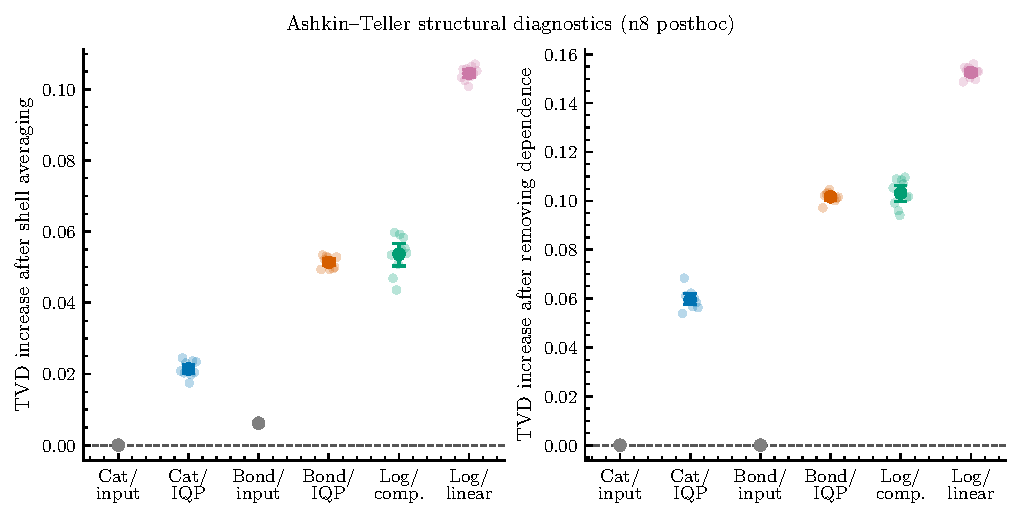
\includegraphics[width=\textwidth]{figures/ashkin_teller_structure_n8.pdf}
 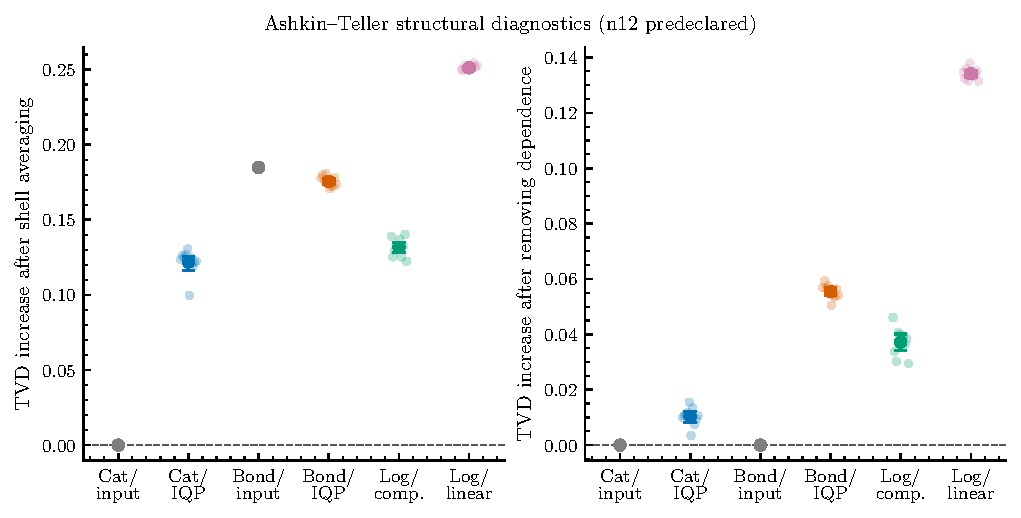
\includegraphics[width=\textwidth]{figures/ashkin_teller_structure_n12.pdf}
 \widefigurecaption{Spatial and dependence diagnostics for all six models at $n=8$ (top, post hoc) and $n=12$ (bottom, predeclared). Faint points show seed means, solid points show the mean and bars show percentile 95\% bootstrap intervals. Grey encoder-only controls are deterministic. Left: TVD change after redistributing mass uniformly within each joint layer-weight shell. Right: TVD change after replacing the joint output by the product of its full layer marginals. Positive values mean the original output is closer to the target than its transformed distribution; these changes do not measure improvement over the input. The transformations are defined in Appendix~\ref{app:at-diagnostics}. Seed means can be positive while individual condition deltas are negative; all condition results are retained in the accompanying artifacts.}{fig:at-structure}
\end{minipage}
\end{plainwidetext}
